% Target: 2ish pages \w graphics
\section{Concept}
% Note: mention that in our context load balancing and entry-gateway are sort of equivalent. Show their relation a bit
% Note: Mention that our approach uses the method of using real-life experiments to inform simulation

To understand the approach we first take a step back to view the boarder technical context the solution addresses and is built around.
As previously outlined, our solution aims to improve the performance of network bound workloads.
In the context of serverless edge computing systems network bound workloads are characterized by the network being the main or a significant contributing factor to the overall response time.
\begin{figure}
    \centering
    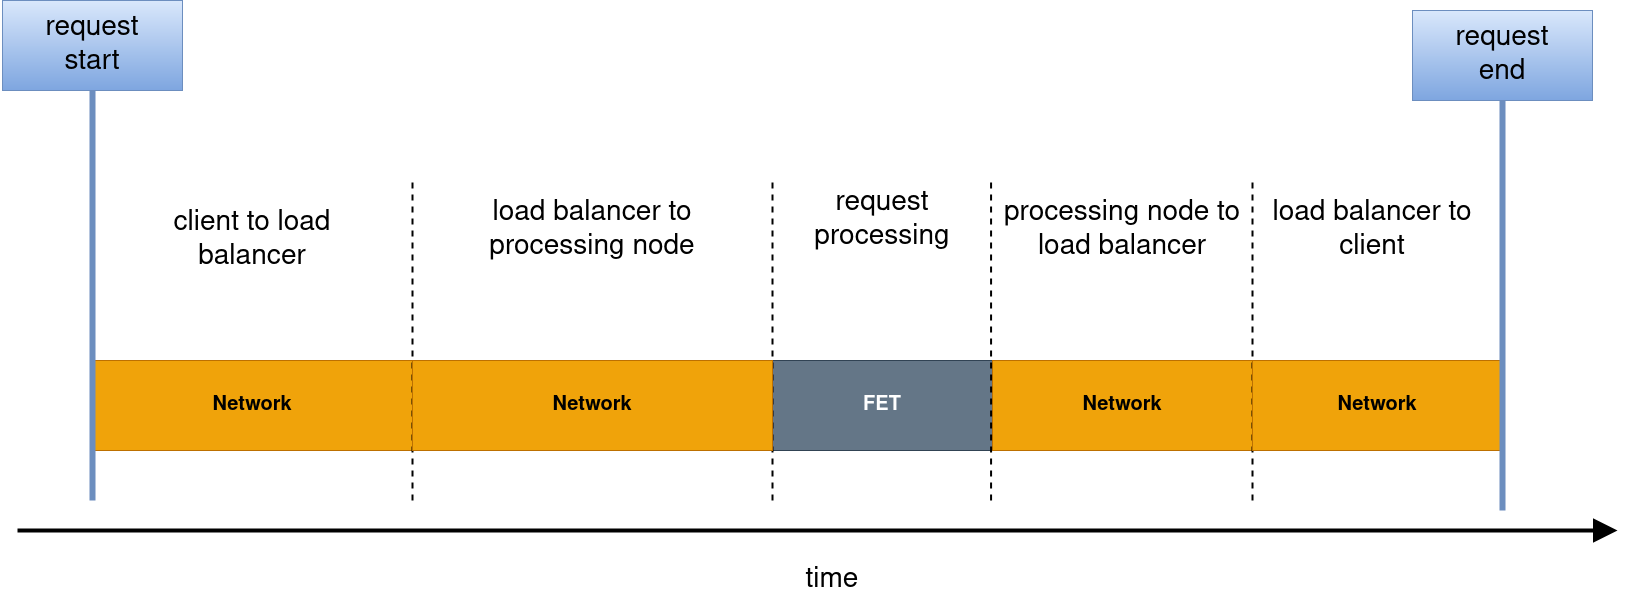
\includegraphics[width=14cm]{graphics/diagrams/request_overview.png}
    \caption{A generic view of the different parts that make up the total request processing time from the perspective of our approach}
    \label{fig:request_net_fet_overview}
\end{figure}
In Figure \ref{fig:request_net_fet_overview} we can see the different processing steps we consider for a request.
A network bound workload in this sense is one where the time taken up by the network portion of handling the request is proportionally speaking significantly larger than the portion taken by the \gls{fet}.
This is typically the case because the request either contains a lot of data that needs to be transported, or because the \gls{fet} is very short.

The primary way by which our approach improves the response times of network bound workloads is thus by reducing the amount of time spent on the network transfer portion of handling a client request.
While optimizing \glspl{fet} is not the primary objective of our approach, at least from a systems design perspective, it still has the potential to additionally reduce \glspl{fet} compared to current methods.
We consider the structure and makeup of the serverless computing system to be a given factor. As a result our approach aims to reduce network times not by changing the network makeup itself, but by utilizing the existing resources as effectively as possible. From a network-optimization perspective this means that each request should take an optimal path from  the client to the node where the request is ultimately processed. 

\begin{figure}
    \centering
    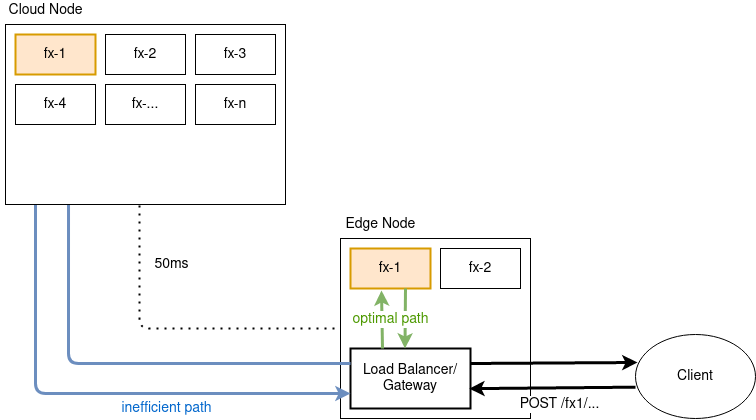
\includegraphics[width=12cm]{graphics/diagrams/efficient_path_example.png}
    \caption{Example diagram showing efficient and inefficient request routing based on network delay. "fx-1" through "fx-2" denote different types of function, and the dotted line denotes a network link between the cloud and edge node with a latency of 50ms}
    \label{fig:efficient_path}
\end{figure}

As can be understood quite intuitively in Figure \ref{fig:efficient_path}, round robin load balancing will in many cases lead to clearly suboptimal choices in terms of incurred network delay. The figure also shows the three key components we consider when trying to make network location based decisions: The client, the load balancer, and the node. Because our approach solely considers application level load balancers, since serverless platforms typically require these for their advanced routing decisions, any given request takes a path from the client to the load balancer, then to the selected upstream node, and back the same way.

Subsequently we want to incur the minimal amount of delay possible from both the hop between the client and load balancer, as well as between the load balancer and upstream node. Our proposed approach handles these two kinds of hops separately, at least for the most part. Since the scope of this work does not include optimizing the location of the serverless function instances themselves, this means we can improve performance through the following methods:
\begin{enumerate}
    \item \textbf{Intelligent load balancing decisions:} load balancers should choose upstream nodes that are both close in the network, and have \glspl{fet} short enough as not to negate the performance won through network proximity
    \item \textbf{Effective placement of load balancers:} the scheduler of the serverless system should place load balancers at locations in the network where they are in close proximity to clients and serverless function instances requested by these clients
    \item \textbf{Efficient scaling of load balancers:} the number of load balancers should be high enough to provide the needed performance improvement, but not so high that the resources consumed by the load balancers diminish or even negate that effect
\end{enumerate}
In our approach the first method is provided by the load balancer itself. It is continuously updated with information where function instances, typically also referred to as \textit{replicas}, are located. Based on this and other information gathered by the load balancer, it tries to make decisions that lead to faster overall request responsiveness by selecting upstreams that are close and provide fast \glspl{fet}.

The other two methods are handled by the osmotic joint scaling and scheduling component of our approach. While the different methods of improvement are split between these two components of our proposed solution, this does not mean that they are completely separate from each other. Naturally the scheduling and scaling decisions will influence the way in which the placed load balancers work, while these in-turn affect the data gathered for and available to the scaling and scheduling component. The specifics of these two components will be discussed in the next two sections. 

It is also important to note that a significant amount of the approaches' implementation details are not chosen arbitrarily, but are rather the result of continuous cycles of experimentation and evaluation. While not detailed in the approach, the evaluation, and discussion chapters of this thesis include some of these experiments, in particular those that give additional insight into the problem domain and yielded results useful beyond informing this specific approach.